\section{Working hours}

The next attack aims to extract information about the working hour behaviour of a target.
This should be achieved by displaying the pattern of the target in form of a weighted scatter plot and by comparing those patterns between several targets.
There are several possible vectors for this attack:

\begin{itemize}
    \item Obtain Information about the sleep rhythm of the target.
    \item Detect whether the target is a person working regular shifts from from Monday to Friday or rather an open-source contributor working in their leisure time.
    \item Detect anomalies such as automated programs, which contribute to a project on a regular basis.
    \item Compare the working hour patterns of several people in the same project or organization. This could, for instance, be used to infer relationships between colleagues, based on an equal working shifts.
\end{itemize}

Additionally a clustering will be performed to find anomalies, common patterns and to evaluate the results of this analysis.
As we are only interested in contributors with a representative amount of commits, all contributors with less than one hundred commits in the last year have been excluded.
This reduced the amount of considered contributors from 175.000 to about 10.300.


\subsection{Implementation}\label{punchcard-implementation}

The data used for this analysis are the commit timestamps of the target, as well as the Github employee information for verification.
These commit timestamps are then converted into a different format, which represents the occurrences of commit per hour per weekday over the last year.
The result is a simple vector with length 168, which corresponds seven days with 24 hours each.
I will refer to this representation hereafter as a \emph{punchcard}.

\begin{minted}[linenos]{python}
def preprocess(commits):
    punchcard = [0] * 168
    for commit in commits:
        hour = commit.commit_time.hour # returns 0-23
        weekday = = commit.commit_time.weekday() # returns 0-6

        index = weekday*24 + hour
        punchcard[index] += 1

\end{minted}
\begingroup
\captionof{listing}{Data preprocessing}\label{lst:puchcard-preprocessing}
\endgroup

The data transformation is simply achieved by incrementing the field of the respective weekday and hour by one for each commit, as can be seen in~\ref{lst:puchcard-preprocessing}.
The resulting punchcard vector is then stored in the database for faster and easier analysis in the next steps.

\begin{figure}[H]
    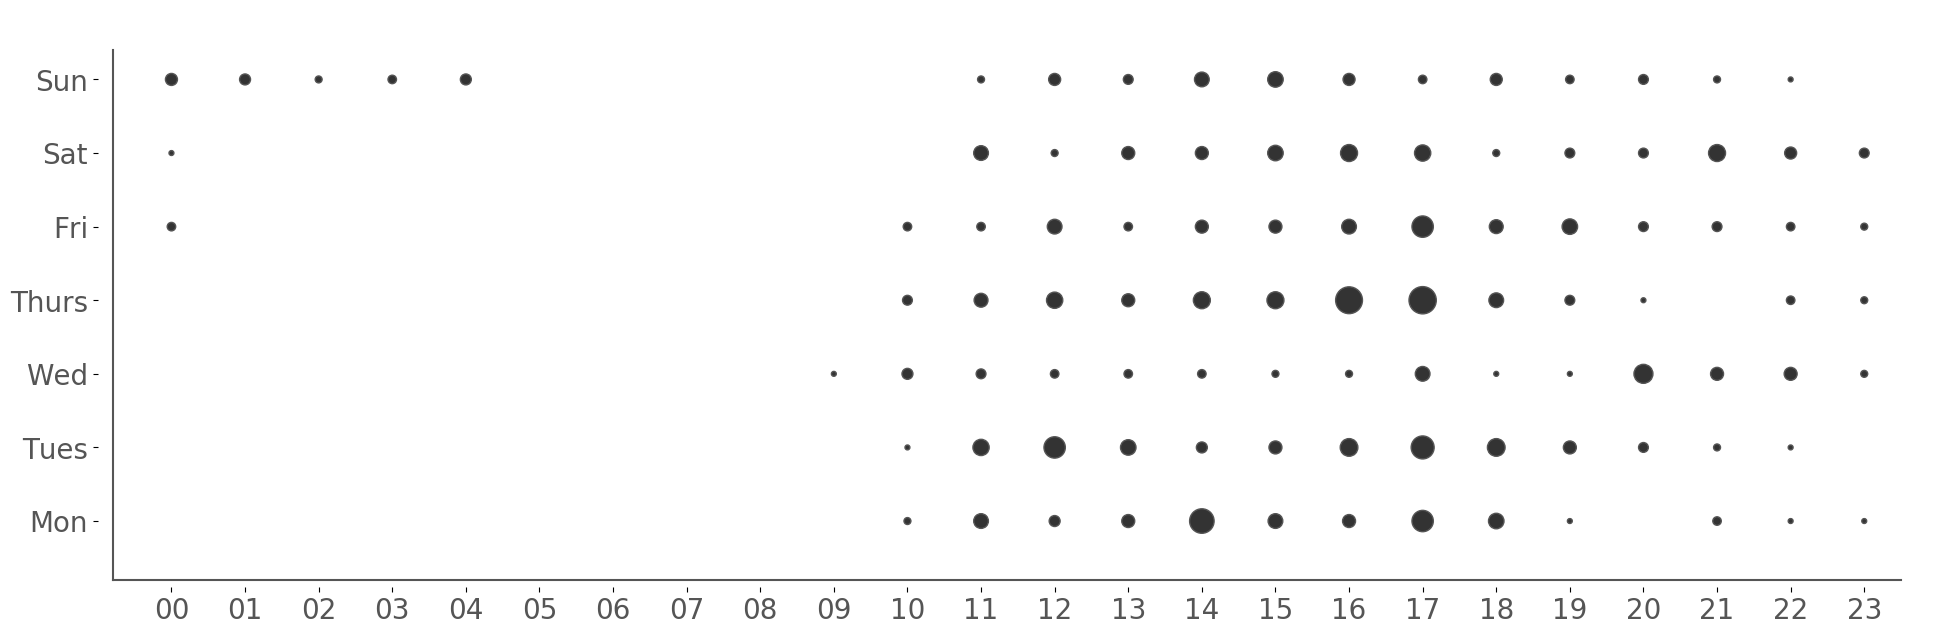
\includegraphics[scale=0.32]{./graphs/analysis/ordered-punchcard}
    \centering
    \caption{Punchcard of the author.}\label{fig:working-hour-rhythm-author}
\end{figure}


\subsection{Punchcard Clustering}

To find common work patterns, several cluster algorithms have been used on the aggregated data.
The Python \emph{scikit} framework has been used for this purpose, as it features nine different clustering methods and provides good documentation and abstraction from the underlying clustering logic~\footnote{`Clustering' scikit-learn.org, http://scikit-learn.org/stable/modules/clustering.html (accessed, 24.04.2018)}.

For the task of finding similar punchcard patterns in the data, a clustering algorithm is required, which can operate on a high-dimensional dataset with an unknown amount of clusters
Scikit provides three different clustering algorithms, which can handle an unknown amount of clusters.

\subsubsection{Mean Shift}\label{mean-shift}
Mean shift is a clustering methods, which performs an operation similar to a gradient descent, by which all adjacent data points are shifted towards their center~\cite{article:mean-shift}.
The goal of this algorithm is to find a representative centroid for each cluster and assign each data point to a cluster.
Unfortunately this methodology proves to be too aggressive for the current data.

\begin{figure}[H]
    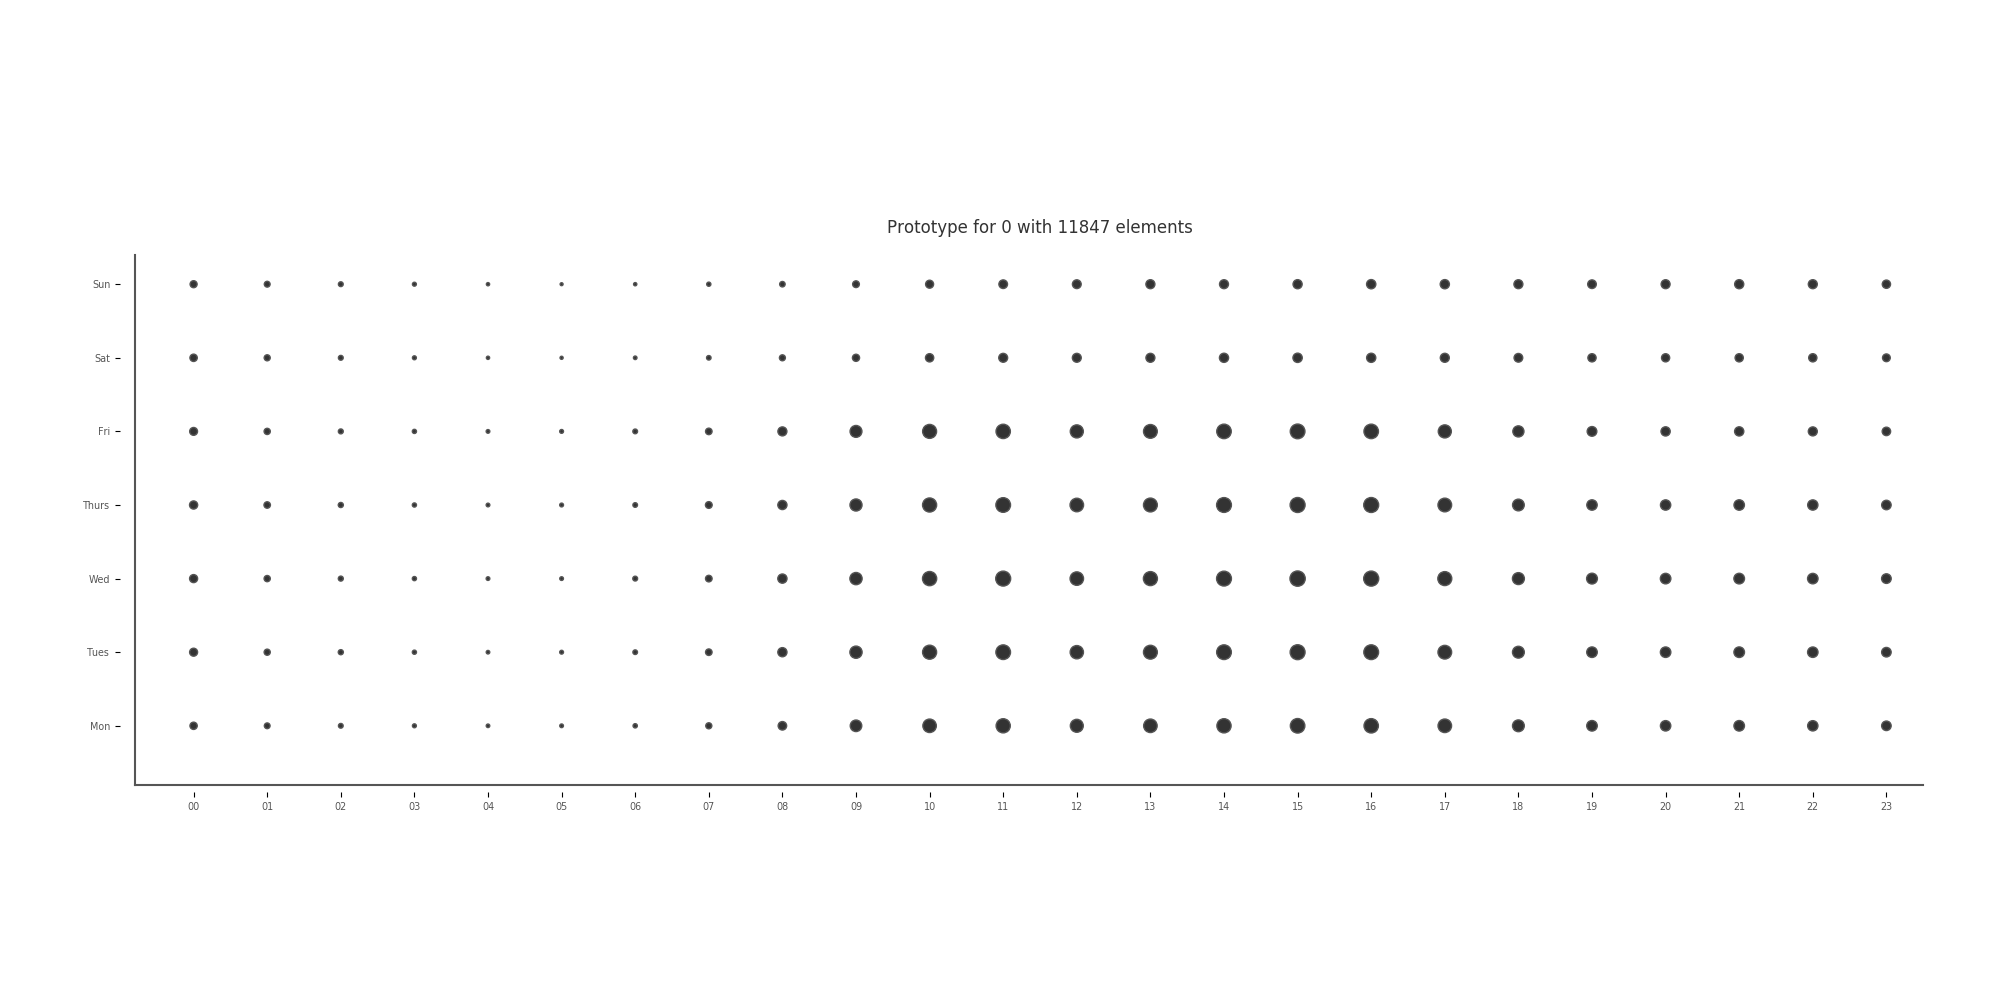
\includegraphics[scale=0.32]{./graphs/analysis-mean-shift/supercluster}
    \centering
    \caption{Super cluster centroid found by mean-shift clustering.}\label{fig:mean-shift-super-cluster}
\end{figure}

Despite trying a wide range of values for the bandwidth, which is the measure of distance used for detecting adjacent points, this algorithm always created a super cluster, which containes more than 89\% of all data points.
Such a super cluster can be seen in Figure~\ref{fig:mean-shift-super-cluster}.
The other 11\% were invariably small clusters representing extreme outlier or strange patterns, which do not resemble any of the expected patterns for normal work shift or leisure time developers.
An example for such an extreme outlier can be seen in Figure~\ref{fig:mean-shift-outlier}.

My assumption is, that the density of data points is too high and that they are too equally distributed around the centroid of the super cluster, for the major part of the provided data.
Thereby all those data points are slowly shifted to this single centroid.
As it is difficult to debug 168-dimensional space, I decided that a profound analysis would be too time consuming and to try the next solution.

\begin{figure}[H]
    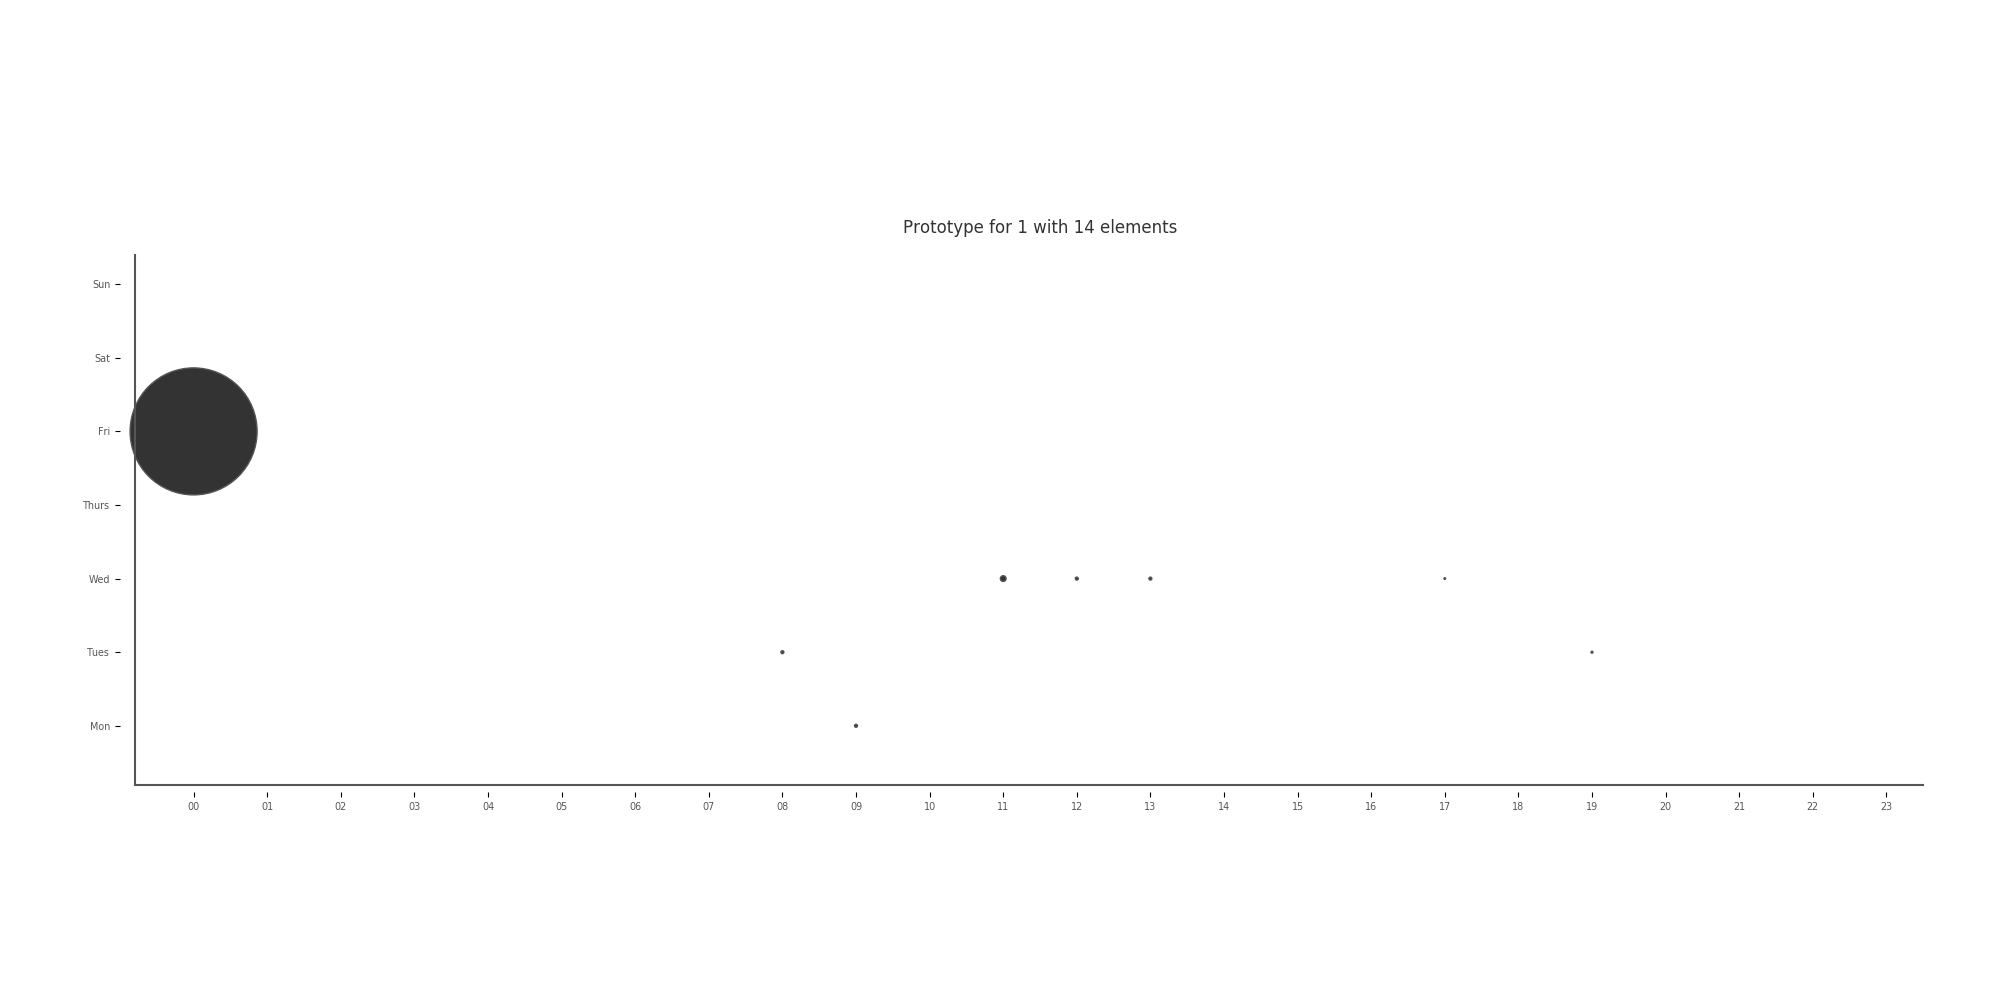
\includegraphics[scale=0.32]{./graphs/analysis-mean-shift/outlier}
    \centering
    \caption{Extreme outlier centroid found by mean-shift clustering.}\label{fig:mean-shift-outlier}
\end{figure}

\subsubsection{DBSCAN}
The \ac{dbscan} clustering algorithm operates by creating clusters of transitively connectable data points within a specific maximal acceptable distance between adjacent points.~\ref{inproceedings:dbscan}.
It is highly scalable and performant, even for large data sets, which made it my first choice.
Unfortunately it produces very similar results to the mean shift clustering algorithm~\ref{mean-shift}, since it finds a super cluster very similar to Figure~\ref{fig:mean-shift-super-cluster}.

I assume that this algorithm suffers from similar problems as the mean shift approach, which are high density and equal distribution of data points without clear borders.
Thereby the algorithm manages to reach the most part of all data points transitively from a single starting point.
When supplied with smaller values for the maximal acceptable distance between data points, it creates a huge amount of mini clusters, just as expected.

This algorithm also manages to find extreme outlier clusters, but it is not suitable for the purpose of this thesis, due to the extremely low granularity on the data inside the super cluster.


\subsubsection{Affinity Propagation}
The Affinity Propagation algorithm considers similarities between all data points to find clusters~\cite{article:affinity-propagation}.
This clustering algorithm features a promising approach, as it utilizes a method similar to message passing, to find an \emph{exemplar}, which resembles the representative of a cluster, and its surrounding cluster member.

Affinity Propagation was the only available clustering method that was detailed enough to find interesting patterns without creating a super cluster.
About 200 different patterns have been discovered using this methodology.
However it has to be noted, that this clustering method is sometimes a little too detailed, since it split very similar patterns into two or more different clusters.

Additionally, the memory requirements for this algorithm scale quadratically for non-sparse sets with the number of the data points~\cite[p.~ii]{article:affinity-propagation}.
About 12 \ac{gb} memory have already been used with a sample of roughly 10.000 data points.
This algorithm becomes thereby impractical for analyses on the whole dataset, but it works for smaller analyses and is thereby suitable for the validation of this thesis.
